\chapter{Megvalósítás C\# programozási nyelven}

A térkép generálásához az alkalmazást C\# programozási nyelven készítettem el. Az objektum orientált elvek figyelembe vételével a programot logikailag különálló osztályokra bontottam szét. Ezek hierarchiája, egymással való kapcsolatai egy az adathordozón mellékelt ábrán láthatóak.

A különböző osztályokat és működésüket a következő pontokban fogom bemutatni, kisebb logikailag összetartozó egységek alapján a könnyebb átláthatóság érdekében.

\begin{figure}[h!]
\centering
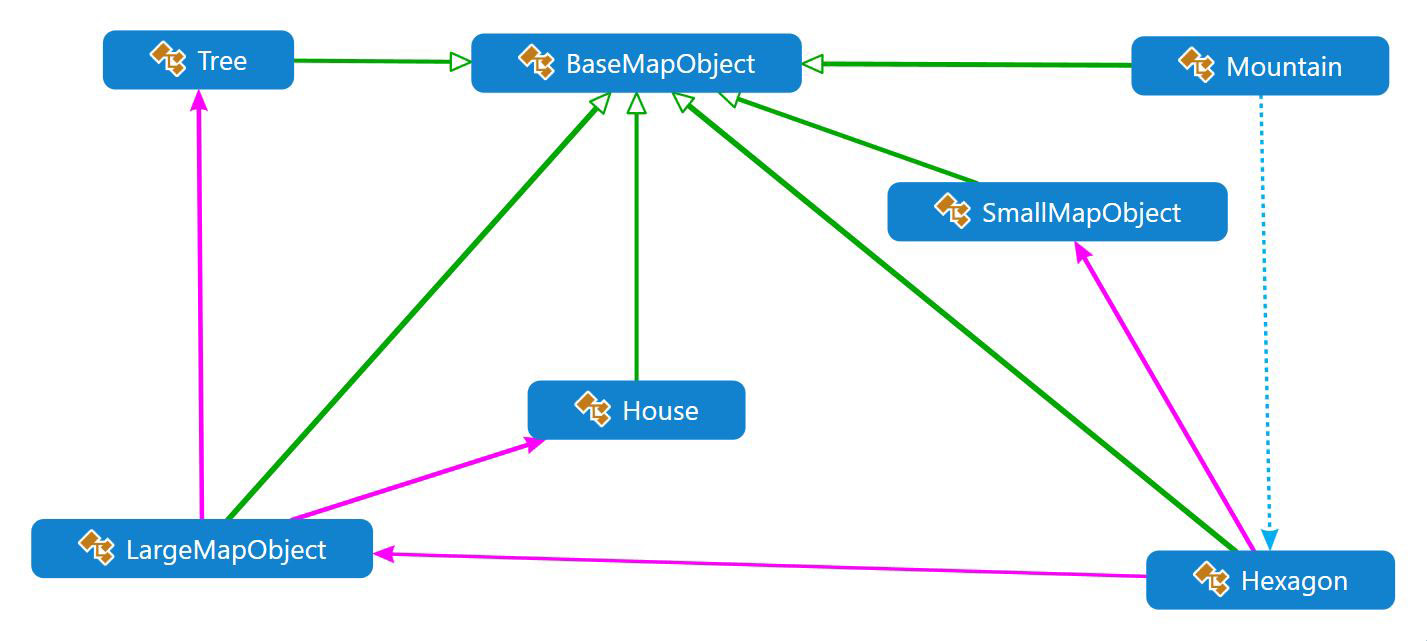
\includegraphics[scale=0.3]{kepek/White_modellek.JPG}
\caption{A programban szereplő modellek hierarchiája}
\label{fig:modellek}
\end{figure}

\section{Modellek kezeléséhez szükséges osztályok}

A \texttt{BaseMapObject} osztályból származik az összes modellekhez kapcsolt osztály. Ez írja le a közös tulajdonságaikat, a térképen szereplő objektumok pozícióját, típusát, azt hogy kiválasztható mezőről van-e szó. A térképen megjelenő objektumokhoz kapcsolt osztályokat a \texttt{Hexagon} osztály kapcsolja össze. Ez az osztály tárolja  a hexagonhoz tartozó statikus hőmérsékletet, vízszintet és amikor változás áll be az aktuális hőmérsékletben, akkor meghívja a hozzá kapcsolt objektumoknak a megfelelő metódusait. A kisebb objektumok (virág, kaktusz, kő) és a nagyobb objektumok (épületek, fák) a \texttt{LargeMapObjectManager} és \texttt{SmallMapObjectManager} osztályokkal kezelhetők.

Minden egyes hexagon modell egy \texttt{Map} elnevezésű üres objektum leszármazottjaként jön létre. Az összes többi modell pedig a \texttt{Hexagon} leszármazottja. Ezáltal könnyebben kereshetőek az objektumok a Unity API-k segítségével.

A \texttt{Tree} osztályban egy tömbben megadható a fa modelleknek azok a részei, amik a lombot alkotják. Az algoritmus pedig a környezeti viszonyoknak megfelelően módosítja (szabályozza a láthatóságát vagy az évszaknak megfelelően módosítja a színeket).

Az épületek esetében is a fáknál már megismert módszert alkalmaztam arra, hogy szabályozzam a környezeti viszonyoknak a behatását az épületekre vonatkozóan.

Manager osztályokat hoztam létre amikben tömbökben megadhatóak a textúrák és az anyagjellemzők (\textit{material}), ezeket az inspector panelen lehet megadni (\ref{fig:Managers}. ábra).

\begin{figure}[h!]
\centering
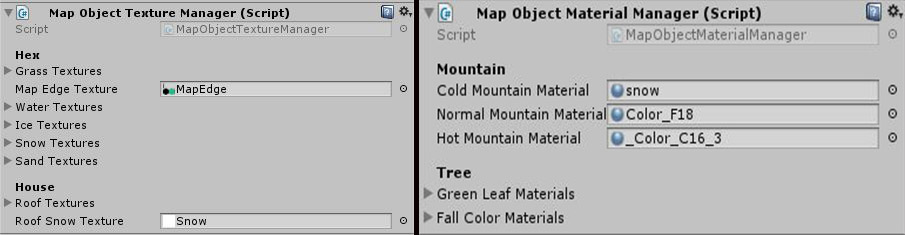
\includegraphics[scale=0.45]{kepek/Managers.jpg}
\caption{Manager osztályok állítási lehetősége az Inspector panelen}
\label{fig:Managers}
\end{figure}

\section{UI és paraméterek szabályozása}

A felhasználói felületen található vezérlő elemek segítségével szabályozhatjuk a generálni kívánt térkép paramétereit. Minden vezérlő elemhez tartozik egy script fájl, ami a játék indításakor beállítja a vezérlő elemekhez tartozó alapértéket és bizonyos esetekben a minimum, maximum vagy a további lehetséges értékeket is. Ezek az értékek az \texttt{Engine} osztályban kerültek rögzítésre. A paraméterek aktuális értékét az \texttt{Engine} megfelelő metódusainak meghívásával lehet módosítani (\ref{fig:UI} ábra.).

\begin{figure}[h!]
\centering
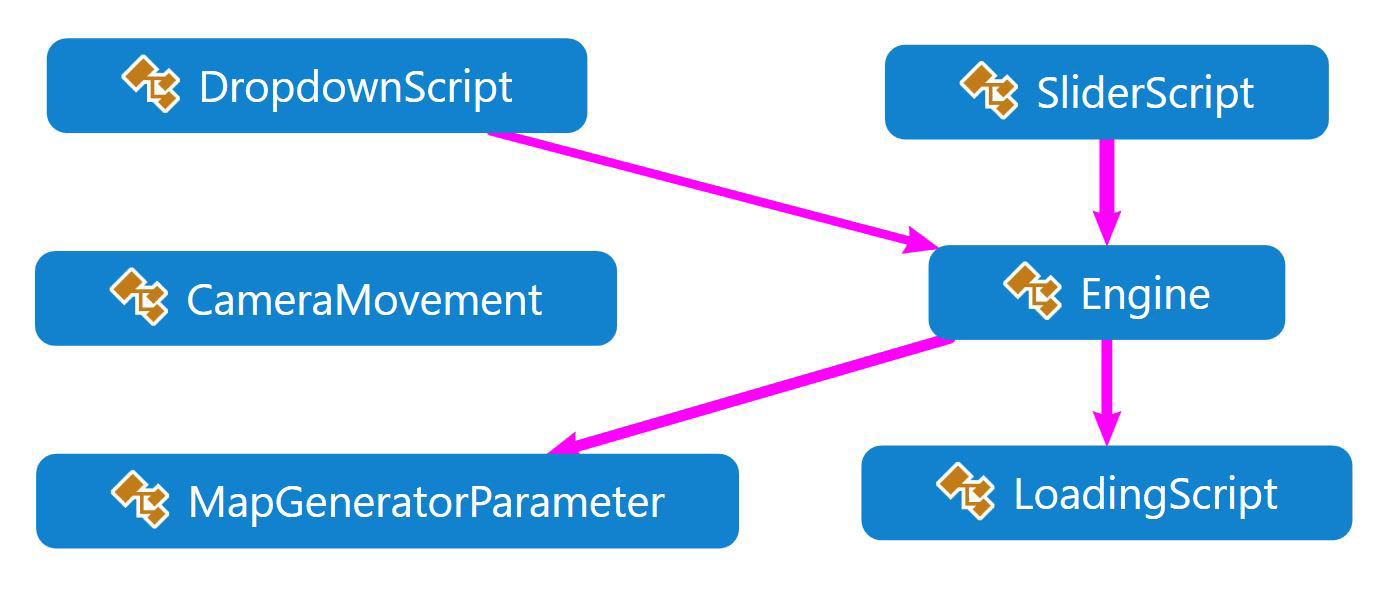
\includegraphics[scale=0.3]{kepek/White_UI.JPG}
\caption{A felhasználói felülethez kapcsolódó osztályok és az Engine kapcsolata}
\label{fig:UI}
\end{figure}

A \texttt{CameraMovement} osztály felelős a kamera mozgatásért. Ennek az osztálynak a kódját a \textit{Unity store}-ból szereztem be \cite{RTS_Camera}, mivel minden alapvető kritériumnak megfelelt amit terveztem és csak apróbb módosításokra volt szükségem (tengelyeken való mozgás limitálásának kiegészítése). 

\begin{figure}[h!]
\centering
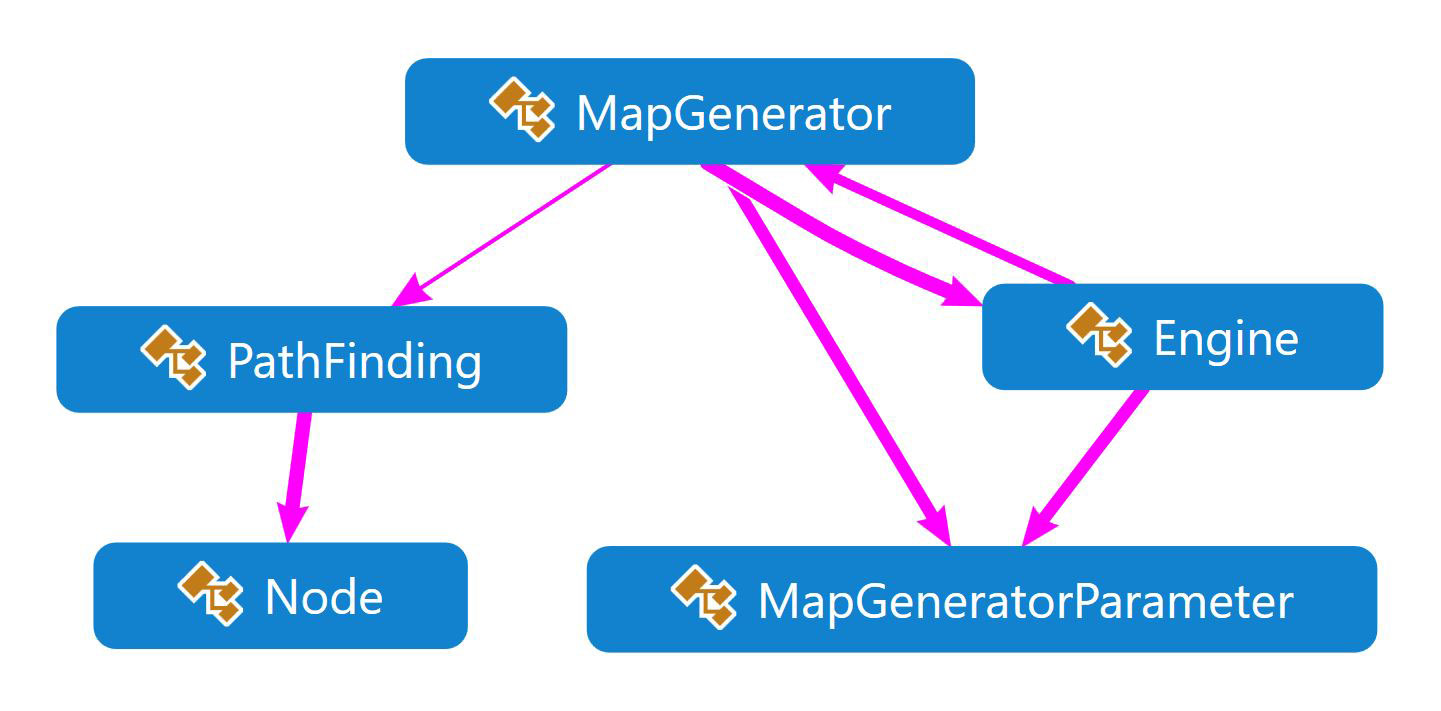
\includegraphics[scale=0.3]{kepek/White_Generalas.JPG}
\caption{Generálási folyamathoz kapcsolódó főbb osztályok}
\label{fig:generalas}
\end{figure}

\newpage

A \texttt{MapGenerator} osztály az, ami a generálást elvégzi. Ennek \aref{chap:tervezes}. fejezetben már ismertetett 8 lépés alapján (\ref{fig:generalas}. ábra).

\subsection{Térkép szélének generálása}

Jelenlegi állapotában a térképet csak valamilyen speciális textúrájú hexagonnal lehet körülhatárolni, de jövőbeli igény esetén minimális módosítások által elérhető lesz más objektumok használata is. A térkép széleinek generálási módját az alábbi kód részletezi.
\begin{cpp}
for (int x = 0; x < map.GetLength(0); x++)
{
   CreateTile(this.transform, new Vector3(x, 0, 0),
   TileTypes.MapEdge, SelectionInfoTypes.NonSelectable);
   CreateTile(this.transform, new Vector3(x, 0, map.GetLength(1) - 1),
   TileTypes.MapEdge, SelectionInfoTypes.NonSelectable);
}

for (int y = 0; y < map.GetLength(1); y++)
{
   CreateTile(this.transform, new Vector3(0, 0, y),
   TileTypes.MapEdge, SelectionInfoTypes.NonSelectable);
   CreateTile(this.transform, new Vector3(map.GetLength(0) - 1, 0, y),
   TileTypes.MapEdge, SelectionInfoTypes.NonSelectable);
}
\end{cpp}

\subsection{Domborzat generálása}

A domborzat generálása véletlenszerű pozíciókba történik, amely konkrétan az alábbi kóddal került megvalósításra.
\begin{cpp}
int maxNumOfMountainTiles = 
(int)(Engine.Instance.MapWidth.Value * Engine.Instance.MapHeight.Value * 
(Engine.Instance.MountainPercent.Value / 100.0));

System.Random rnd = new System.Random();

int i = 0;
while (i < maxNumOfMountainTiles)
{
   Vector3 position = new Vector3
   (
      rnd.Next(1, map.GetLength(0) - 1),
      0, rnd.Next(1, map.GetLength(1) - 1)
   );

   if (map[(int)position.x, (int)position.z] == null)
   {
      CreateTile
      (
         this.transform, position, TileTypes.Mountain, 
         SelectionInfoTypes.ChildObject
      );
      i++;
   }
}
\end{cpp}

\subsection{Folyók generálása}

A folyók generálásához \textit{A*-algoritmus}t használtam. A nagy terjedelmű algoritmus helyett csak a pszeudokódot mutatnám be, ami alapján implementáltam ezt a részt \cite{A*Code}.
\begin{cpp}
OPEN 
CLOSED 
add the start node to OPEN

loop
   current = node in OPEN  with the lowest f_cost
   remove current from OPEN
   add current to CLOSED

   if current is the target node
      return

   foreach neighbour of the current node
      if neighbour is not traversable or neighbour is in CLOSED
         skip to the next neighbour

      if new path to neighbour is shorter OR neighbour is not in OPEN
         set f_cost of neighbour
         set parent of neighbour to current
         
         if neighbour is not in OPEN
            add neighbour to OPEN
\end{cpp}

Fontosnak tartom még megemlíteni azt, hogy az algoritmus során szükséges tárolnunk minden egyes csomópontról, hogy melyik csomópontról értük el. Amikor vizsgálunk egy csomópontot, akkor az összes szomszédját megvizsgáljuk, hogy rajta vannak-e valamelyik listán. Ha már rajta van a lezárt listán akkor tovább lépünk a következőre, viszont, ha a vizsgálandó csomópontok listáján szerepel, akkor meg kell, hogy vizsgáljuk, hogy az aktuálisan vizsgált csomópontról nem rövidebb-e az út mint a korábbi útvonal volt.

\subsection{További mezők generálása}

További mezők generálása alatt jelen esetben olyan mezők generálását értjük, amelyeken nem szerepel folyó vagy hegy, de szerepelhetnek rajta épületek vagy növények. Ennek a generálási módja a következő kódrészben olvasható.
\begin{cpp}
for (int y = 0; y < map.GetLength(1); y++)
{
   for (int x = 0; x < map.GetLength(0); x++)
   {
      if (map[x, y] == null)
      {
         CreateTile(this.transform, new Vector3(x, 0, y),
         TileTypes.Flat, SelectionInfoTypes.Selectable);
         OpenFlatTiles.Add(new Vector2(x, y));
      }
   }
}

MaxNumOfCities = (int)(OpenFlatTiles.Count * 
(Engine.Instance.CityPercent.Value / 100.0));
MaxNumOfBiome = (int)(OpenFlatTiles.Count * 
(Engine.Instance.BiomePercent.Value / 100.0));
\end{cpp}

A szabad mezők nyilvántartásba vételére azért van szükség, hogy a generálás későbbi szakaszaiban tudjuk, hogy mennyi épületet vagy növényzetet kell generálni.

\subsection{Épületek generálása}

Az alábbi algoritmus véletlenszerűen kiválasztott mezőkre generál épületeket/városokat a korábban meghatározott mértékben.
\begin{cpp}
if (OpenFlatTiles.Count > 0)
{
   int numOfCities = 0;
    
   while ( (numOfCities < MaxNumOfCities) && (OpenFlatTiles.Count > 0))
   {
      Vector2 index = OpenFlatTiles[UnityEngine.Random.Range(0, 
      OpenFlatTiles.Count)];

      map[(int)index.x, (int)index.y].GetComponent<Hexagon>
      ().AddMapObject(HexagonComponents.LargeMapObject, 
      LargeMapObjectTypes.City);
      numOfCities++;
      OpenFlatTiles.Remove(index);
   }
}
\end{cpp}

\subsection{Növényzet generálása}

Ebben a pontban azt az algoritmust mutatom be, amelyik meghatározza, hogy a szabad mezők közül melyikre és milyen növényzetet generáljon.
\begin{cpp}
if (OpenFlatTiles.Count > 0)
{
   int numOfSmall = 0;
   int numOfLarge = 0;

   while ( (numOfSmall < MaxNumOfBiome || numOfLarge < MaxNumOfBiome )
   && (OpenFlatTiles.Count > 0) )
   {
      Vector2 index = OpenFlatTiles[UnityEngine.Random.Range(0, 
      OpenFlatTiles.Count)];
                
      int hexComponentIndex = 0;

      if (map[(int)index.x, (int)index.y].GetComponent
      <SmallMapObjects>() != null)
      {
         hexComponentIndex += 1;
      }
      if (map[(int)index.x, (int)index.y].GetComponent
      <LargeMapObjects>() != null)
      {
         hexComponentIndex += 2;
      }

      switch (hexComponentIndex)
      {
         case 0:
            if (UnityEngine.Random.Range(0, 2) == 0)
            {
               map[(int)index.x, (int)index.y].GetComponent
               <Hexagon>().AddMapObject(HexagonComponents.SmallMapObject, 
               LargeMapObjectTypes.Trees);
               numOfSmall++;
            }
            else
            {
               map[(int)index.x, (int)index.y].GetComponent
               <Hexagon>().AddMapObject(HexagonComponents.LargeMapObject, 
               LargeMapObjectTypes.Trees);
               numOfLarge++;
            }
            break;
         case 1:
            map[(int)index.x, (int)index.y].GetComponent
            <Hexagon>().AddMapObject(HexagonComponents.LargeMapObject, 
            LargeMapObjectTypes.Trees);
            numOfLarge++;
            break;
         case 2:
            map[(int)index.x, (int)index.y].GetComponent
            <Hexagon>().AddMapObject(HexagonComponents.SmallMapObject, 
            LargeMapObjectTypes.Trees);
            numOfSmall++;
            break;
         case 3:
            OpenFlatTiles.Remove(index);
            break;
      }
   }
}
\end{cpp}
